\documentclass[11pt]{article}

\usepackage[strings]{underscore}
\usepackage{amsmath}
\usepackage{graphicx}
\usepackage{amssymb}

\begin{document}

\section*{Question 1}
\subsection*{Part A}

The logistic loss function for labels \{-1,1\} is the same as the logistic function for labels \{0,1\}. 
Proof as show in~\cite{logisticloss} is summarized below.

Given that the logistic function is:
\begin{equation}
		P(y=1 | \theta, x) = \frac{1}{1+e^{-\theta^Tx}}
		\label{eq:logistic}
\end{equation}

It can be shown that given Eq(\ref{eq:logistic}), we can show that: 
\begin{equation}
		P(-x) = 1 - P(x)
\label{eq:property2}
\end{equation}
\begin{equation}
		P(y=0 | \theta, x) = \frac{e^{-\theta^Tx}}{1+e^{-\theta^Tx}}
\end{equation}

For the logistical loss function:
\begin{equation}
		P(y | \theta, x) = \frac{1}{1+e^{-y\theta^Tx}}
		\label{eq:loss}
\end{equation}

The equations are equivalent for $y=1$. For $y=0$, it can be shown that $P(y=0|\theta, x)$ and 
$P(y=-1|\theta,x)$ are equivalent through Property~\ref{eq:property2}. We could also show that
this leads to the same decision boundary. We define the boundary for logistic regression as:
\begin{align}
		\begin{split}
				\frac{\frac{1}{1+e^{-\theta^Tx}}}{\frac{e^{-\theta^Tx}}{1+e^{-\theta^Tx}}} &> 1 \rightarrow y=1 \\
		\theta^Tx &> 0 
		\end{split}
\end{align}

Likewise the boundary for logistic loss can be written as:
\begin{align}
		\begin{split}
				\frac{\frac{1}{1+e^{-\theta^Tx}}}{\frac{1}{1+e^{\theta^Tx}}} &> 1 \rightarrow y=1 \\
		\theta^Tx &> 0
		\end{split}
\end{align}

Given the logistical loss function~\ref{eq:loss}, we would try to maximize the probability of a vector of 
observed results $y$ with the likelihood function:
\begin{align}
		\begin{split}
				L(\theta) &= p(\vec{y}| \theta; X) \\
				&=\prod_{i=1}^{m}p(y^{(i)}|\theta;x^{(i)}) \\
				&=\prod_{i=1}^{m}\frac{1}{1+e^{-y\theta^Tx}}
		\end{split}
\end{align}

Taking the log likelihood and maximizing:
\begin{align}
		l(\theta) = -\sum_{i=1}^{m}log(1+e^{-y\theta^Tx})
\end{align}

This is a similar form to the one provided in the question. Maximizing the log likelihood is also minimizing
the loss function $\sum_{i=1}^{m}log(1+e^{-y\theta^Tx})$, which can be found in ~\cite{logisticloss}.

Getting back to the question at hand, to show that the Hessian $H$ is positive semidefinite, we 
differentiate $J(\theta)$ twice:
\begin{align}
		\begin{split}
	g(z) &= \frac{1}{1+e^{-z}} \\
		g(y\theta^Tx) &= \frac{1}{1+e^{-y^{(k)}\theta^Tx^{(k)}}}
		\end{split}
\end{align}
\begin{align}
		\begin{split}
		\frac{\partial J'(\theta)}{\partial \theta_j} &= -\frac{1}{m}\sum_{i=1}^{m}\frac{1}{g(y^{(k)}\theta^Tx^{(k)})}g'(y^{(k)}\theta^Tx^{(k)})y^{(k)}x^{(k)}_j \\
		&= -\frac{1}{m}\sum_{i=1}^{m}(1-g(y^{(k)}\theta^Tx^{(k)}))y^{(k)}_jx^{(k)}_j \\
		&= -\frac{1}{m}\sum_{i=1}^{m}y^{(k)}x^{(k)}_j-g(y^{(k)}\theta^Tx^{(k)})y^{(k)}x^{(k)}_j \\
		\frac{\partial J''(\theta)}{\partial \theta_j \partial \theta_i} &= -\frac{1}{m}\sum_{i=1}^{m}-y^{(k)}x^{(k)}_jg(y^{(k)}\theta^Tx^{(k)})y^{(k)}x^{(k)}_i \\
																		 &= \frac{1}{m}\sum_{i=1}^{m}y^2x_ix_j[g(y\theta^Tx)(1-g(y\theta^Tx))]
		\end{split}
\end{align}

Note in the last equation, we dropped the index k for clarity. Further since $z^THz$ can be re-expressed as:
\begin{align}
		\begin{split}
		z^THz &= \sum_{i}\sum_{j}(x_{ij}z_j)z_i \\
		&= \sum_{i}\sum_{j}z_i[\frac{1}{m}\sum^{m}y^2g(y\theta^Tx)(1-g(y\theta^Tx))]x_ix_jz_j
		\end{split}
\end{align}

Note that $\frac{1}{m}\sum^{m}y^2g(y\theta^Tx)(1-g(y\theta^Tx))$ is always greater than zero since $y^2 \geq 0$ and $0 \leq g(y\theta^Tx) \leq 1$. 
Therefore, we only need to prove that $\sum_{i}\sum_{j}z_ix_ix_jz_j>0$. We can do this by:
\begin{align}
		\begin{split}
		\sum_{i}\sum_{j}z_ix_ix_jz_j &= \sum_{i}x_iz_i\sum_{j}x_jz_j \\
		&= (x^Tz)^2 \geq 0 
		\end{split}
\end{align}

But why does proving semi-definite-ness prove convexity? We begin with the definition of convexity.

\textbf{Definition 1.} A function $f: \mathbb{R}^n \rightarrow \mathbb{R}$ is convex if its domain 
is a convex set and for all $x_1$, $x_2$ in its domain, and all $\lambda \in [0,1]$, we have:
\begin{align}
	f(\lambda x_1+(1-\lambda)x_2) \leq \lambda f(x_1) + (1-\lambda)f(x_2)
\end{align}

This equation says that an equation $f$ is convex in the range $[x_1, x_2]$ if you can draw a line between 
$f(x_1)$ and $f(x_2)$ such that the function $f$ will always be smaller than that. A more detailed 
graphical interpretation can be found in~\cite{convexity}.

We first prove \textbf{Lemma 1:} $f(x_2) \geq f(x_1) + \nabla f(x_1)^T(x_2-x_1)$, then $f$ is 
convex~\cite{characterConvexity}. 
We let $z=\lambda x_2 + (1-\lambda)x_1$. 
\begin{align}
	\begin{split}
		f(z)-f(x_1) \leq \lambda f(x_2) + (1-\lambda)f(x_1) - f(x_1) = \lambda f(x_2) - \lambda f(x_1)
	\end{split}
\end{align}

We know that the gradient $\nabla f(x_1)^T(x_2-x_1)$ can be re-expressed as
\footnote{Here $\nabla f(x_1)^T(x_2-x_1)$ is a first-order directional derivative with expansion 
shown in along with why first/second-order expansion over can be substituted by $z \in [x_1,x_2]$
~\cite{directionalDerivative}}:

\begin{align}
	\begin{split}
		\nabla f(x_1)^T(x_2-x_1) &= \lim_{\lambda \rightarrow 0^+}\frac{f(x_1+\lambda(x_2-x_1))-f(x)}{\lambda} \\
		&= \lim_{\lambda \rightarrow 0^+}\frac{f(z)-f(x)}{\lambda} \leq f(x_2) - f(x_1)
	\end{split}
\end{align}

This implies that:
\begin{align}
	f(x_2) \geq f(z) + \nabla f(z)^T(x_2-z) \\
	f(x_1) \geq f(z) + \nabla f(z)^T(x_1-z) \\
\end{align}

Which if we multiply the first equation by $\lambda$ and second by $(1-\lambda)$ and sum both equations, 
given that we had let $z=\lambda x_2 + (1-\lambda)x_1$,  we would arrive at the definition of convexity in
\textbf{Definition 1}.

Using \textbf{Lemma 1}, we can take the taylor expansion of $f(x_2)$:
\begin{align}
	\begin{split}
	f(x_2) = f(x_1) + \nabla f(x_1)^T(x_2-x_1) + \frac{1}{2}((x_2-x_1)^TH(z)(y-x)) \\
	\implies f(x_2) \geq f(x_1) + \nabla f(x_1)^T(x_2-x_1) \\ 
	\textnormal{if H is positive semidefinite}
	\end{split}
\end{align}
By extension of \textbf{Lemma 1}, semi-definiteness therefore proves convexity. 


\subsection*{Part B}

The co-efficient of the fit is [ 0.76037154  1.17194674 -2.6205116 ].

Several interesting caveats were discovered through mistakes. First, initially no parameter for
y-intercept was learned. This produced pretty good results, but was 5\% worse in accuracy than
parameters that included a y-intercept (-2.6205116 above). 

Second, a programming mistake in calculating gradient resulted in labels that were suppose to be
{-1} to be assigned as {1} and vice versa. Interestingly this produced the same boundary. The
mistake was calculating $g(y^{(k)}\theta^Tx)y_j^{(k)}x_j^{(k)}$ instead of the correct  
$(1-g(y^{(k)}\theta^Tx))y_j^{(k)}x_j^{(k)}$. At first, I thought this was because I may have 
assigned the labels to probability wrong, so I simply reversed the mappings to threshold. 
However, after working through the math a bit more, I realized I did the mapping to label 
correct, but somehow I was getting 12\% accuracy when I assign $h(\theta^Tx)>0.5 y\rightarrow1$.
Upon closer inspection, the error was found.

\subsection*{Part C}
\begin{figure}
	\centering
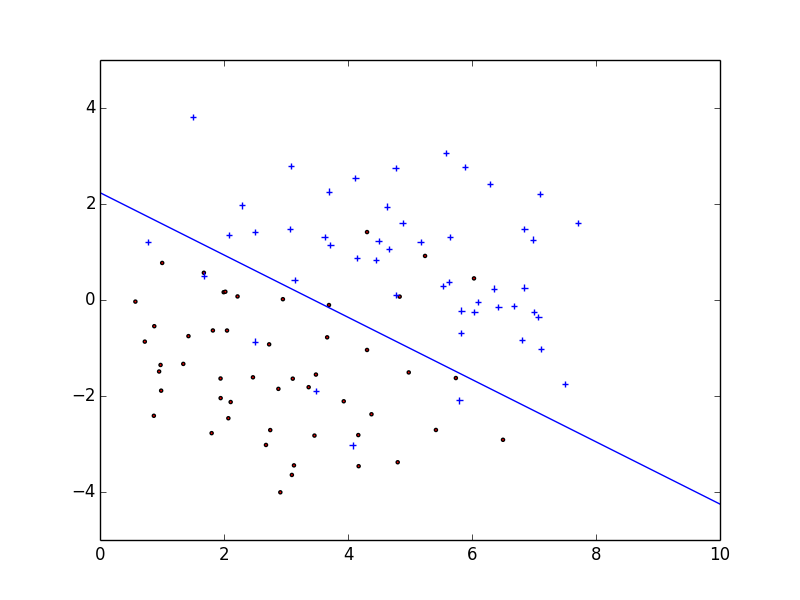
\includegraphics[width=0.75\textwidth]{../p1.png}
	\caption{ '+' indicate \{1\} labels and '.' indcate \{-1\} labels.}
	\label{fig:1c}
\end{figure}

See Figure~\ref{fig:1c}.



\bibliographystyle{abbrv}
\bibliography{solutions}

\end{document}
